% ======================================================================
% RESULTS PACK: proto results-and-discussion chapter (LIVING DRAFT)
% Deep Reinforcement Learning for Optimal Order Execution on Real
% Hyperliquid Order-Book Data
%
% Status: WORKING DRAFT assembled 2026-07-17 for supervisor review.
% This document is deliberately comprehensive (every result included;
% curation to the final dissertation set happens at report assembly,
% with overflow moving to appendices). It is NOT frozen: sections will
% be revised as the remaining pre-registered experiments complete.
%
% Overleaf usage: upload the figures/ folder next to this file; all
% tables are inlined below, so this single file plus figures/ compiles.
% ======================================================================
\documentclass[11pt]{article}
\usepackage[margin=2.4cm]{geometry}
\usepackage{graphicx}
\usepackage{booktabs}
\usepackage{amsmath}
\usepackage{caption}
\usepackage{longtable}
\usepackage[colorlinks=true, linkcolor=blue, urlcolor=blue]{hyperref}
\usepackage{xcolor}
\graphicspath{{figures/}}
\captionsetup{font=small, labelfont=bf}
\setlength{\parskip}{4pt}

\newcommand{\statusbox}[1]{\begin{center}\fcolorbox{black}{yellow!12}{\parbox{0.93\textwidth}{\small \textbf{Status:} #1}}\end{center}}

\title{Results and Discussion (Working Draft)\\
\large Deep Reinforcement Learning for Optimal Order Execution on Real Hyperliquid Order-Book Data}
\author{Fardeen Idrus}
\date{19 July 2026}

\begin{document}
\maketitle

\noindent\emph{Working draft: every result produced so far is included at this stage; the
selection of material and the prose will be revised in later dissertation stages as the
remaining pre-registered experiments complete.}

\section{Experimental architecture}\label{sec:arch}

\subsection{Two complementary tracks}

The study asks whether deep reinforcement learning (DRL) agents can execute a large buy
order in Bitcoin more cheaply than time-weighted average price (TWAP) scheduling, and it
answers this on two complementary experimental tracks built from the same underlying market:
Hyperliquid BTC-USD order-book data from December 2025.

\begin{enumerate}
\item \textbf{The frozen-replay track.} Agents trade against replayed historical order-book
snapshots (1-minute and 10-second bars). The market contains every empirical predictive
signal that was present in the data, but it cannot react to the agent: the agent's own
trades do not move the replayed prices. This track therefore measures whether
\emph{signal-timing} skill exists, under the assumption of negligible market impact.
\item \textbf{The reactive-simulator track.} Agents trade inside a queue-reactive model
(QRM) calibrated on per-order (L4) BTC data, in which the agent's market orders consume
real book liquidity, move the price, and interact with calibrated refill dynamics. Two
regime-specific calibrations are used (calm and volatile). This track measures whether
\emph{impact-management} skill exists, in a market that reacts.
\end{enumerate}

Together the tracks cover the two mechanisms by which an execution agent could beat TWAP;
each track holds the other's mechanism fixed. The reactive-simulator track is the study's
main focus; the frozen-replay track is a secondary strand whose chief role is to motivate the
move to a reacting market (Section~\ref{sec:l2}). A pre-registered extension that combines both
mechanisms in one environment (the measured-signal extension, Section~\ref{sec:next}) is
designed and queued.

\subsection{Environment validation (reactive simulator)}

Before any agent was trained, the reactive simulator had to pass pre-registered validation
gates. Table~\ref{tab:t5} reports the gates of record after the background-drift correction
described below: the agent's own impact is real and persistent on the relevant horizon
(an identical order submitted immediately after the first costs roughly $2.4\times$ as
much, because the first has consumed the visible liquidity and the book has not yet
refilled), dump costs are size-monotone, the book demonstrably refills, simulated
cost-versus-size growth tracks the real books within the pre-registered band, and the TWAP
benchmark completes $100\%$ of episodes.

A material confound was found and corrected at this stage: the December 2025 calibration
month was directionally rising, and replaying it na\"ively gave every fast-buying policy a
mechanical advantage. The background move process was therefore drift-neutralised (volatility
preserved), and a permanent fairness gate was added: the residual drift is statistically zero
in both regimes, and no constant-pace policy is significantly cheaper than TWAP (maximum
$|t| = 1.77$ across all pace multiples and regimes). Figure~\ref{fig:drift} shows the
before-and-after effect on an identical 20-run design retrained under the corrected
process: the apparent calm-regime advantage shrinks from $-0.019$\,bps to an immaterial
$-0.006$\,bps, statistically indistinguishable from zero across seeds (95\% confidence
interval $[-0.020, +0.010]$) and an order of magnitude below the $0.05$\,bps economic
materiality floor adopted below.

\begin{table}[h]\centering\small
\caption{Environment validation gates of record after drift correction. Rows one to
three verify that the agent's own trading genuinely moves the simulated market and that the
book both remembers and recovers from the impact; row four that simulated cost growth with
order size matches the real order book; rows five and six that the TWAP benchmark operates
correctly and that immediate execution is properly penalised; the final two rows that the
corrected background process gives no schedule a mechanical advantage. Archived records:
\texttt{step4\_gates\_v3.json} and \texttt{step3g/fairness\_verdict\_*.json}, in which these
checks carry the internal identifiers G1$'$, G2, G3 and the fairness gate, in row order.}
\label{tab:t5}
\resizebox{\textwidth}{!}{% Auto-generated from step4_gates_v3.json + step3g/fairness_verdict_*.json.
\begin{tabular}{llllc}
\toprule
regime & check & measured & pass band & verdict \\
\midrule
calm & own impact is real and persists (2nd immediate dump / 1st, cost ratio) & 2.41 & $\geq 1.25$ & PASS \\
calm & dump cost increases with order size (Spearman $\rho$) & 1.00 & $> 0$ & PASS \\
calm & book refills after impact (probe cost $+30$s vs $+1$s, bps) & -0.46 vs 0.35 & lower at $+30$s & PASS \\
calm & cost-vs-size growth matches the real book (sim vs real ratio) & 2.45 vs 2.46 & within band & PASS \\
calm & fixed-TWAP completes every episode & 100\% & $\geq 99\%$ & PASS \\
calm & dumping costs more than scheduling (dump / TWAP, drift-free, bps) & 0.40 / 0.20 & dump $\geq$ TWAP & PASS \\
calm & no residual background drift (ticks/episode; $t$) & 0.12 ($t$=0.27) & $t$ n.s. & PASS \\
calm & no constant-pace policy beats TWAP (max $|t|$ across paces) & 1.42 & none significant & PASS \\
volatile & own impact is real and persists (2nd immediate dump / 1st, cost ratio) & 2.35 & $\geq 1.25$ & PASS \\
volatile & dump cost increases with order size (Spearman $\rho$) & 1.00 & $> 0$ & PASS \\
volatile & book refills after impact (probe cost $+30$s vs $+1$s, bps) & -0.23 vs 0.14 & lower at $+30$s & PASS \\
volatile & cost-vs-size growth matches the real book (sim vs real ratio) & 2.44 vs 1.99 & within band & PASS \\
volatile & fixed-TWAP completes every episode & 100\% & $\geq 99\%$ & PASS \\
volatile & dumping costs more than scheduling (dump / TWAP, drift-free, bps) & 0.24 / 0.05 & dump $\geq$ TWAP & PASS \\
volatile & no residual background drift (ticks/episode; $t$) & 0.07 ($t$=0.06) & $t$ n.s. & PASS \\
volatile & no constant-pace policy beats TWAP (max $|t|$ across paces) & 1.77 & none significant & PASS \\
\bottomrule
\end{tabular}}
\end{table}

\begin{figure}[h]\centering

\includegraphics[width=0.78\textwidth]{fig6_drift_confound.pdf}
\caption{The drift confound. The identical 20-run base campaign evaluated with the
original background process (grey) and after drift-neutralisation (blue); the design is
identical and the agents are retrained under each background process. Open circles are
individual seeds, diamonds the group mean with 95\% confidence interval, and the horizontal
line marks adaptive-TWAP parity. After neutralisation the apparent calm-regime advantage
shrinks from $-0.019$\,bps to an immaterial $-0.006$\,bps, statistically indistinguishable
from zero (the 95\% confidence interval spans zero) and an order of magnitude below the
pre-registered $0.05$\,bps materiality floor, while the volatile group moves within seed
noise. The residual-drift and constant-pace checks of Table~\ref{tab:t5} confirm the
corrected background gives no schedule a mechanical advantage.}
\label{fig:drift}
\end{figure}

\subsection{Evaluation machinery}

\textbf{Paired evaluation with common random numbers (CRN).} Every policy (agent and both
benchmarks) is evaluated on the same 2{,}000 episodes with identical episode seeds, so
market luck cancels in the paired per-episode differences and the comparison isolates
policy skill.

\textbf{Two TWAP benchmarks, both required.} The fixed benchmark is the textbook open-loop
schedule (order$/N$ per decision, with fractional-unit carry). The adaptive benchmark
re-plans the remaining quantity over the remaining time each second; it is exactly the
agent's ``always $1.0\times$ pace'' action, so it is the neutral element of the agent's own
action space and the industry-realistic implementation. The pre-registered edge definition
requires beating \emph{both}; the adaptive benchmark is the headline metric because it is
the stricter of the two. At the primary setting the choice is empirically immaterial, with
the two benchmarks agreeing to within $0.001$ basis points (bps) per seed. At the smallest
order size in the robustness grid (5\,BTC) the two schedules genuinely diverge, by up to
$0.08$\,bps per seed, which is one more reason the edge definition requires beating both.
No verdict in this document changes under either benchmark.

\textbf{Frozen decision rules.} The definition of ``beats TWAP'' was frozen before any run:
per-seed Wilcoxon signed-rank $p<0.01$ against both benchmarks, the sign consistent in at
least four of five seeds, and a pooled advantage of at least $0.05$\,bps (an economic
materiality floor, since CRN pairing can make trivially small differences statistically
significant; $0.05$\,bps is approximately $1\%$ of one taker fee). A lower investigation
tripwire (pooled $\leq -0.02$\,bps with across-seed $p<0.05$) guarantees that a
small-but-consistent effect is never silently discarded: it triggers a pre-registered
follow-up instead.

\textbf{Three-layer evaluation.} Because roughly 200 trained configurations were screened
against the same development episodes, the design inserts a replication layer between
screening and confirmation, analogous to discovery and replication cohorts in genomics or
public and private leaderboards in machine-learning competitions: (1) \emph{screen} on the
development block; (2) \emph{replicate} candidates on a never-before-used reserve block
after escalating to five seeds; (3) \emph{confirm} survivors on a sealed block used exactly
once. Figure~\ref{fig:pipeline} summarises the architecture and what happened at each layer.
The replication layer was added, dated and documented, after the first two sealed tests
failed; its first use (Section~\ref{sec:robust}) justified it emphatically.

\begin{figure}[h]\centering
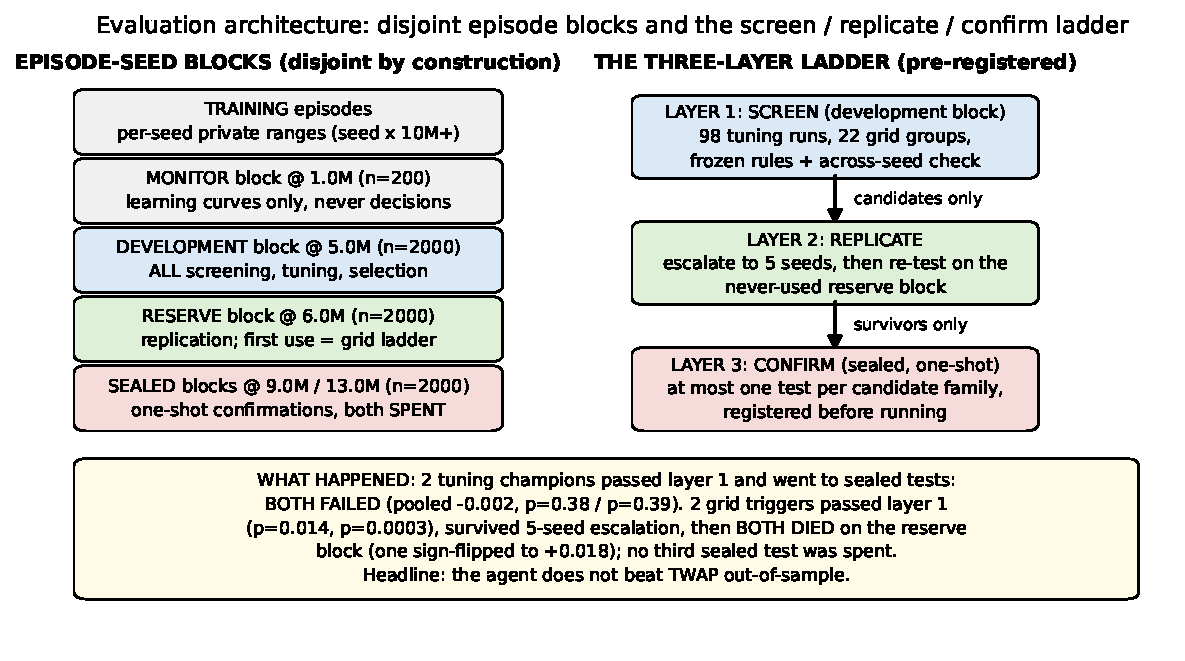
\includegraphics[width=0.98\textwidth]{fig22_pipeline_schematic.pdf}
\caption{Evaluation architecture. Each evaluation block is a disjoint set of episode
random seeds, so no two blocks share market paths. Roughly 200 trained configurations were
screened on the development block; groups meeting the pre-registered trigger were escalated
to five seeds and replicated on the never-before-used reserve block; only selection winners
reached the single-use sealed blocks. The diagram records what happened at each layer.}
\label{fig:pipeline}
\end{figure}

\clearpage
\section{Research question 1: can DRL beat TWAP in a reacting market?}\label{sec:rq1}

We trained PPO and DQN agents to buy 25 BTC in five minutes inside
the reactive simulator, tuned them extensively, and sent the two best configurations to
one-shot sealed tests. Neither survived. The headline result of this study is a
\emph{boundary null}: a development-block advantage that repeatedly fails to exist on fresh
data.

\subsection{Primary campaign}

Twenty agents (PPO and DQN, calm and volatile regimes, five seeds each; 2M training steps;
identical $30{\times}5$ networks and matched gradient sample throughput of ${\sim}20$M
sample-passes per run) were evaluated under the frozen rules. Table~\ref{tab:t1} gives every
run. No cell met the edge definition. All ten PPO agents passed the behaviour audit; seven
of ten DQN agents collapsed (Section~\ref{sec:dqn}). The volatile-regime PPO group showed
the strongest sub-threshold signal: five of five seeds cheaper than both benchmarks, pooled
$-0.047$\,bps, across-seed $p=0.006$. Figure~\ref{fig:regime} shows the contrast
directly. For base PPO and the later-selected variant alike, the calm-regime seeds cluster
at the benchmark line while the volatile-regime seeds sit consistently below it;
Section~\ref{sec:rq2} returns to this regime split once the confirmation verdicts are in
hand.

\begin{table}[h]\centering\small
\caption{Primary campaign, all 20 runs. Source: \texttt{step5\_v3/}.}
\label{tab:t1}
\resizebox{0.86\textwidth}{!}{% Auto-generated from step5_v3/judgement.json + behaviour_audit.json. Do not edit by hand.
\begin{tabular}{llrrrrc}
\toprule
algo & regime & seed & vs fixed-TWAP & $p_{\mathrm{fix}}$ & vs adaptive-TWAP & valid \\
 & & & (bps) & & (bps) & \\
\midrule
dqn & calm & 0 & +0.1124 & 0.015 & +0.1125 & \textbf{NO} \\
dqn & calm & 1 & +0.0596 & 0.072 & +0.0597 & \textbf{NO} \\
dqn & calm & 2 & +0.0263 & 0.326 & +0.0264 & \textbf{NO} \\
dqn & calm & 3 & +0.1533 & 0.000 & +0.1534 & \textbf{NO} \\
dqn & calm & 4 & -0.0016 & 0.829 & -0.0015 & yes \\
dqn & volatile & 0 & +0.4176 & 0.001 & +0.4169 & \textbf{NO} \\
dqn & volatile & 1 & -0.0296 & 0.632 & -0.0303 & yes \\
dqn & volatile & 2 & +0.3017 & 0.003 & +0.3011 & \textbf{NO} \\
dqn & volatile & 3 & -0.0389 & 0.383 & -0.0396 & yes \\
dqn & volatile & 4 & -0.0197 & 0.893 & -0.0203 & \textbf{NO} \\
ppo & calm & 0 & -0.0108 & 0.958 & -0.0107 & yes \\
ppo & calm & 1 & +0.0110 & 0.576 & +0.0111 & yes \\
ppo & calm & 2 & -0.0194 & 0.324 & -0.0193 & yes \\
ppo & calm & 3 & +0.0020 & 0.597 & +0.0020 & yes \\
ppo & calm & 4 & -0.0108 & 0.632 & -0.0107 & yes \\
ppo & volatile & 0 & -0.0317 & 0.350 & -0.0324 & yes \\
ppo & volatile & 1 & -0.0357 & 0.442 & -0.0364 & yes \\
ppo & volatile & 2 & -0.0892 & 0.012 & -0.0898 & yes \\
ppo & volatile & 3 & -0.0319 & 0.417 & -0.0326 & yes \\
ppo & volatile & 4 & -0.0433 & 0.444 & -0.0439 & yes \\
\bottomrule
\end{tabular}}
\end{table}

\begin{figure}[h]\centering

\includegraphics[width=0.75\textwidth]{fig8_regime_comparison.pdf}
\caption{Regime dependence of the development-block signal (research question 2). Base
PPO and the selected variant evaluated per regime on the development block; open circles
are individual seeds, diamonds the group mean with 95\% confidence interval. The apparent
advantage was volatile-regime-only and later failed both sealed tests; the calm regime
shows nothing after the drift fix.}
\label{fig:regime}
\end{figure}

\subsection{Hyperparameter search and selection}

Twelve pre-registered PPO variants and two DQN collapse-remediation variants were screened
(98 runs in total; Table~\ref{tab:t2} summarises the groups; the full run-level record is
Appendix Table~A.1; configurations in Table~\ref{tab:t8}). In the volatile regime
seven of eight healthy variants reproduced a small consistent advantage
(Figure~\ref{fig:forestv}); in the calm regime nothing was consistent
(Figure~\ref{fig:forestc}). The selected configuration (learning rate $10^{-3}$, all else
base) pooled $-0.063$\,bps with across-seed $p=0.0043$ on five seeds.

\begin{figure}[h]\centering

\includegraphics[width=0.82\textwidth]{fig3_forest_tuning_volatile.pdf}
\caption{Tuning screen, volatile regime. Each row is one pre-registered variant, labelled
by its single change from the base configuration; open circles are individual seed means on
the development block, the whisker spans the seed range, the diamond is the group mean, and
the dashed line is the $-0.05$\,bps materiality floor. Seven of eight healthy variants sit
below zero, an in-sample consistency later shown to be shared evaluation-block luck.}
\label{fig:forestv}
\end{figure}
\begin{figure}[h]\centering

\includegraphics[width=0.82\textwidth]{fig14_forest_tuning_calm.pdf}
\caption{Tuning screen, calm regime, same layout as Figure~\ref{fig:forestv}. No variant
shows a consistent advantage; seed ranges straddle the benchmark throughout.}
\label{fig:forestc}
\end{figure}

\begin{table}[h]\centering\small
\caption{Tuning and selection, all 28 groups. Source: \texttt{step5\_selection\_v3/}.}
\label{tab:t2}
\resizebox{0.9\textwidth}{!}{% Auto-generated from step5_selection_v3. Do not edit by hand.
\begin{tabular}{lllrrr}
\toprule
variant & change & regime & valid/total & pooled vs adaptive & across-seed \\
 & & & seeds & (bps) & $p$ \\
\midrule
\_v3a & learning rate 1e-3 & volatile & 5/5 & -0.0628 & 0.004 \\
\_v3b & learning rate 1e-4 & volatile & 5/5 & -0.0602 & 0.010 \\
\_v2 & reward x100 & volatile & 5/5 & -0.0462 & 0.002 \\
\_v1b & network 128x128 & volatile & 5/5 & -0.0562 & 0.005 \\
\_v5 & n\_steps 8192 & volatile & 5/5 & -0.0485 & 0.006 \\
\_v4a & ent\_coef 0.0 & volatile & 3/3 & -0.0472 & 0.062 \\
\_v4b & ent\_coef 0.05 & volatile & 5/5 & -0.0267 & 0.048 \\
\_v1a & network 64x64 & volatile & 2/3 & -0.0196 & 0.151 \\
\_v6 & reward x100 @ 10M & volatile & 2/3 & -0.0515 & 0.150 \\
\_v6b & lr 1e-4 @ 10M & volatile & 3/3 & -0.0395 & 0.069 \\
\_w3a & net128 + reward x100 & volatile & 3/3 & -0.0620 & 0.016 \\
\_w3b & lr 1e-4 + reward x100 & volatile & 2/3 & -0.0363 & 0.085 \\
\_d1 & DQN eps 0.05+anneal & volatile & 1/3 & -0.0403 & -- \\
\_d2 & DQN reward x100+net64 & volatile & 3/3 & -0.0259 & 0.199 \\
\midrule
\_v3a & learning rate 1e-3 & calm & 3/3 & +0.0013 & 0.528 \\
\_v3b & learning rate 1e-4 & calm & 2/3 & -0.0239 & 0.111 \\
\_v2 & reward x100 & calm & 3/3 & -0.0024 & 0.322 \\
\_v1b & network 128x128 & calm & 3/3 & -0.0211 & 0.140 \\
\_v5 & n\_steps 8192 & calm & 3/3 & -0.0159 & 0.141 \\
\_v4a & ent\_coef 0.0 & calm & 5/5 & -0.0213 & 0.010 \\
\_v4b & ent\_coef 0.05 & calm & 3/3 & -0.0058 & 0.200 \\
\_v1a & network 64x64 & calm & 3/3 & -0.0159 & 0.040 \\
\_v6 & reward x100 @ 10M & calm & 3/3 & +0.0046 & 0.705 \\
\_v6b & lr 1e-4 @ 10M & calm & 3/3 & -0.0108 & 0.214 \\
\_w3a & net128 + reward x100 & calm & 3/3 & -0.0063 & 0.200 \\
\_w3b & lr 1e-4 + reward x100 & calm & 3/3 & -0.0116 & 0.083 \\
\_d1 & DQN eps 0.05+anneal & calm & 1/3 & -0.0068 & -- \\
\_d2 & DQN reward x100+net64 & calm & 0/3 & -- & -- \\
\bottomrule
\end{tabular}}
\end{table}

\subsection{Sealed confirmations: the headline}

Two configurations earned sealed tests. The first (learning rate $10^{-3}$) was chosen on
volatile-regime performance, the metric used during screening. A documented audit of the
selection step then found that the pre-registered selection rule, applied exactly as
written (ranking configurations on performance across both regimes jointly), would have
chosen a different configuration (network $128{\times}128$); that configuration received
the second sealed test, so both readings of the selection rule were confirmed out of
sample. Each champion was retrained on five fresh seeds and evaluated once on its own
never-used sealed block. \textbf{Both failed} (Table~\ref{tab:t3},
Figure~\ref{fig:headline}): pooled $-0.0023$\,bps ($p=0.379$) and $-0.0022$\,bps
($p=0.394$), confidence intervals bracketing zero. The development-block signal, consistent
across five seeds and twelve variants, does not exist out of sample. The two-test family was
closed by pre-registration; the selection-metric question is resolved empirically, since
both candidate champions returned approximately zero.

Undertraining does not explain the failures. Figure~\ref{fig:curves} tracks both
configurations across the full 2M-step training budget on the independent monitor block:
both oscillate slightly above TWAP parity within seed noise, with no sustained improvement
trend in the second half of training. The policies had converged, and the monitor block
never showed the advantage that the development block did; in hindsight this was the first
sign that the advantage belonged to the evaluation episodes rather than to the policies.

\begin{figure}[h]\centering

\includegraphics[width=0.8\textwidth]{fig1_dev_vs_sealed.pdf}
\caption{The headline result. For each champion configuration, the development-block
evaluation that selected it (blue) is shown next to its one-shot sealed evaluation on fresh
seeds and a never-used episode block (red); open circles are individual seeds, diamonds the
mean with 95\% confidence interval, the horizontal line adaptive-TWAP parity. Both sealed
results sit at approximately zero, so the development-block advantage does not exist out of
sample.}
\label{fig:headline}
\end{figure}

\begin{table}[h]\centering\small
\caption{Both sealed confirmations, per seed, with the pass/fail checklist. Source:
\texttt{step5\_confirm\_v3a/}, \texttt{step5\_confirm\_v1b/}.}
\label{tab:t3}
\resizebox{0.9\textwidth}{!}{% Auto-generated from step5_confirm_v3a (9e6) + step5_confirm_v1b (13e6).
\begin{tabular}{lllrrrc}
\toprule
config & sealed block & seed & vs fixed & vs adaptive & $p$ (adaptive) & valid \\
\midrule
faster-learning (v3a) & 9{,}000{,}000 & 5 & +0.0221 & +0.0222 & 0.749 & yes \\
 &  & 6 & -0.0104 & -0.0103 & 0.813 & yes \\
 &  & 7 & +0.0028 & +0.0028 & 0.804 & yes \\
 &  & 8 & -0.0080 & -0.0079 & 0.936 & yes \\
 &  & 9 & -0.0184 & -0.0184 & 0.758 & yes \\
\cmidrule(lr){2-7}
 & \multicolumn{6}{l}{pooled vs adaptive = -0.0023 bps; across-seed $p$ = 0.379; cheaper in 3/5; \textbf{PASS = FALSE}} \\
\midrule
bigger-network (v1b) & 13{,}000{,}000 & 10 & -0.0010 & -0.0019 & 0.650 & yes \\
 &  & 11 & +0.0042 & +0.0033 & 0.953 & yes \\
 &  & 12 & -0.0297 & -0.0306 & 0.294 & yes \\
 &  & 13 & +0.0153 & +0.0144 & 0.491 & yes \\
 &  & 14 & +0.0047 & +0.0038 & 0.961 & yes \\
\cmidrule(lr){2-7}
 & \multicolumn{6}{l}{pooled vs adaptive = -0.0022 bps; across-seed $p$ = 0.394; cheaper in 2/5; \textbf{PASS = FALSE}} \\
\bottomrule
\end{tabular}}
\end{table}

\begin{figure}[h]\centering

\includegraphics[width=0.75\textwidth]{fig5_learning_curves_volatile.pdf}
\caption{Training curves in the volatile regime, evaluated on the independent monitor
block (200 fixed episodes) throughout the 2M-step budget; lines are means over five seeds,
bands one standard deviation across seeds. Both configurations hover slightly above TWAP
parity with no sustained improvement trend, so the sealed failures are not explained by
undertraining.}
\label{fig:curves}
\end{figure}


\subsection{Per-episode cost distributions}

The sealed records store per-run means and significance values; to characterise the full
cost distributions, the twenty primary-campaign agents were replayed deterministically on
the same 2{,}000 CRN episodes, storing every episode's implementation shortfall for the
agent and both benchmarks. The replay's integrity is verifiable: the recomputed paired
means equal the sealed judgement records exactly for all twenty runs.

Two facts stand out (Figure~\ref{fig:dist}, Figure~\ref{fig:paired}, Table~\ref{tab:t6}).
First, the agents' absolute cost distributions are visually indistinguishable from the
benchmarks': execution cost is dominated by market conditions, not by policy, and the
volatile regime widens every distribution by roughly a factor of $2.5$ (standard
deviation $2.35$ to $5.88$\,bps, Table~\ref{tab:t6}). Second, the paired
per-episode differences dwarf their means: the strongest development-block signal
($-0.047$\,bps in the volatile regime) is three orders of magnitude smaller than the
episode-level spread of the paired differences, which is precisely why 2{,}000 paired
episodes and strict multiple-testing discipline are necessary in this domain.

\begin{figure}[h]\centering
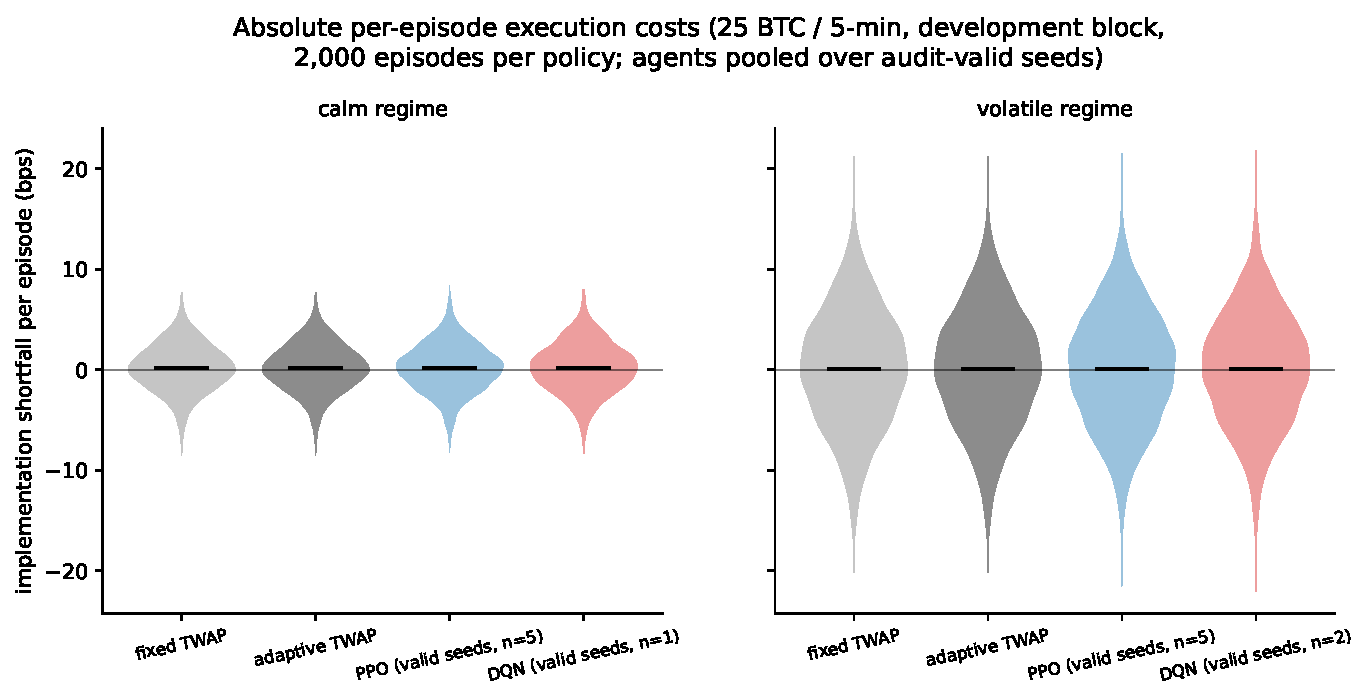
\includegraphics[width=0.98\textwidth]{fig10a_cost_distributions.pdf}
\caption{Absolute per-episode execution costs at the primary setting (development block;
2{,}000 episodes per policy; deterministic replay whose recomputed means match the sealed
records exactly). Each violin is one policy's full cost distribution. Agents and benchmarks
are visually indistinguishable, and the volatile regime widens every distribution by roughly
a factor of $2.5$; market conditions, not policy choice, dominate execution cost.}
\label{fig:dist}
\end{figure}

\begin{figure}[h]\centering
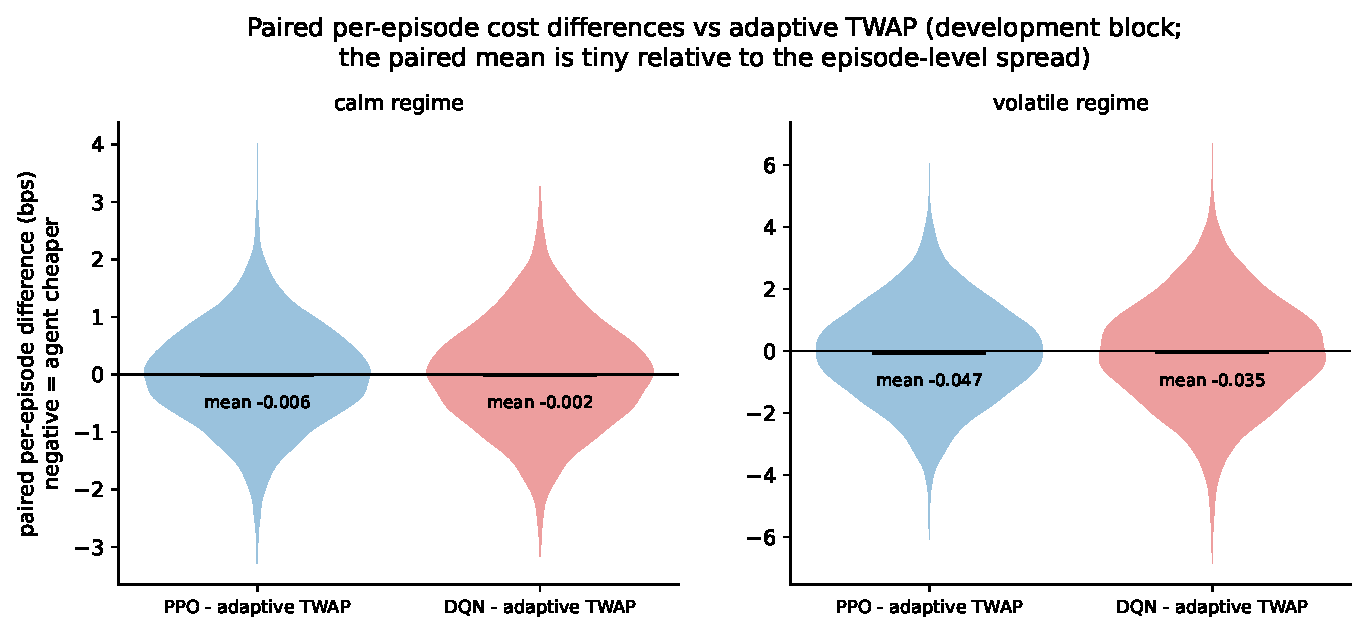
\includegraphics[width=0.98\textwidth]{fig10b_paired_distributions.pdf}
\caption{Paired per-episode cost differences against adaptive TWAP on identical episodes
(negative = agent cheaper). The episode-level spread is roughly three orders of magnitude
larger than the mean differences under test, which is why 2{,}000 paired episodes and strict
significance discipline are needed to measure anything in this domain.}
\label{fig:paired}
\end{figure}

\begin{table}[h]\centering\small
\caption{Descriptive statistics of per-episode costs at the primary setting (bps;
reactive track, development block). Source: \texttt{per\_episode\_v3/}.}
\label{tab:t6}
\resizebox{0.9\textwidth}{!}{% Auto-generated from per_episode_v3/*.npz (deterministic replay; integrity
% exact vs step5_v3/judgement.json for all 20 runs).
\begin{tabular}{llrrrrrr}
\toprule
regime & policy & mean & sd & median & 5\% & 95\% & $n$ episodes \\
\midrule
calm & fixed TWAP & +0.1803 & 2.3546 & +0.1840 & -3.7238 & +4.0427 & 2{,}000 \\
calm & adaptive TWAP & +0.1802 & 2.3540 & +0.1810 & -3.7212 & +4.0245 & 2{,}000 \\
calm & PPO (valid seeds) & +0.1747 & 2.3661 & +0.2089 & -3.7477 & +3.9982 & 10{,}000 \\
calm & DQN (valid seeds) & +0.1787 & 2.4817 & +0.1849 & -3.9363 & +4.2143 & 2{,}000 \\
\midrule
volatile & fixed TWAP & +0.1031 & 5.8800 & +0.1013 & -9.7930 & +9.4489 & 2{,}000 \\
volatile & adaptive TWAP & +0.1037 & 5.8793 & +0.0922 & -9.7133 & +9.4541 & 2{,}000 \\
volatile & PPO (valid seeds) & +0.0567 & 5.7882 & +0.1640 & -9.3214 & +9.2684 & 10{,}000 \\
volatile & DQN (valid seeds) & +0.0688 & 5.6446 & +0.1161 & -9.0810 & +9.1627 & 4{,}000 \\
\bottomrule
\end{tabular}}
\end{table}

\clearpage
\section{Robustness of the null across the design space}\label{sec:robust}

A null at one order size and one deadline could be a blind spot,
so the null was stress-tested across a $4\times4$ grid of order sizes (5 to 50 BTC) and
deadlines (2.5 to 20 minutes), in both regimes. It held everywhere; the two cells that
looked like exceptions died on fresh data, exactly as the earlier illusion had.

\subsection{Order-size response and the full grid}

A genuine impact-management advantage should grow with order size. It does not: the
development-block advantage is non-monotone in size (absent at 5, 12.5 and 50 BTC, present
only at the 25 BTC development size; Figure~\ref{fig:size}), which is the signature of
selection on noise rather than of skill. The full grid (66 new runs; Figure~\ref{fig:grid},
Table~\ref{tab:t4}) is null in 20 of 22 newly tested groups, with several groups
significantly \emph{worse} than TWAP (for example 12.5 BTC at the 20-minute deadline in the
volatile regime, pooled $+0.164$\,bps).

\begin{figure}[h]\centering

\includegraphics[width=0.75\textwidth]{fig2_size_response.pdf}
\caption{Size response of the development-block signal at the 5-minute deadline; points
are group means with 95\% confidence intervals per order size and regime, and the dotted
line marks the 25\,BTC development size. A genuine impact-management advantage should grow
with order size; instead the advantage appears only at the size the configuration was
developed at, the signature of selection on noise.}
\label{fig:size}
\end{figure}

\begin{figure}[h]\centering

\includegraphics[width=0.98\textwidth]{fig9_grid_heatmap.pdf}
\caption{The complete size-by-deadline grid on the development block. Each cell reports
the pooled agent cost versus adaptive TWAP (negative = agent cheaper) with its across-seed
$p$-value. Solid outlines mark the two calm cells that met the pre-registered follow-up
trigger, both of which subsequently died on the reserve block (Figure~\ref{fig:ladder});
the dashed outline marks the volatile centre cell whose signal had already failed both
sealed tests.}
\label{fig:grid}
\end{figure}

\begin{table}[h]\centering\small
\caption{Robustness grid, all 16 cells per regime. Source: \texttt{step5\_grid\_*},
\texttt{step5\_sweep\_*}, \texttt{step5\_selection\_v3}.}
\label{tab:t4}
\resizebox{0.9\textwidth}{!}{% Auto-generated from step5_grid_* + step5_sweep_* + step5_selection_v3. Do not edit.
\begin{tabular}{llrrrrrc}
\toprule
regime & deadline & size & valid/ & cheaper & pooled vs & across-seed & follow-up \\
 & (min) & (BTC) & total & & adaptive (bps) & $p$ & trigger \\
\midrule
calm & 2.5 & 5 & 3/3 & 2/3 & -0.0094 & 0.2498 & no \\
 & 2.5 & 12.5 & 3/3 & 1/3 & +0.0032 & 0.7761 & no \\
 & 2.5 & 25 & 2/3 & 1/2 & +0.0029 & 0.5919 & no \\
 & 2.5 & 50 & 2/3 & 0/2 & +0.0060 & 0.9525 & no \\
 & 5 & 5 & 3/3 & 2/3 & -0.0142 & 0.1346 & no \\
 & 5 & 12.5 & 3/3 & 2/3 & -0.0233 & 0.1191 & no \\
 & 5 & 25 & 3/3 & 2/3 & +0.0013 & 0.5279 & no \\
 & 5 & 50 & 3/3 & 0/3 & +0.0100 & 0.9757 & no \\
 & 10 & 5 & 3/3 & 1/3 & +0.0105 & 0.8819 & no \\
 & 10 & 12.5 & 3/3 & 3/3 & -0.0178 & 0.0261 & no \\
 & 10 & 25 & 3/3 & 3/3 & -0.0250 & 0.0646 & no \\
 & 10 & 50 & 3/3 & 3/3 & -0.0539 & 0.0140 & \textbf{YES} \\
 & 20 & 5 & 3/3 & 0/3 & +0.0338 & 0.9991 & no \\
 & 20 & 12.5 & 3/3 & 1/3 & +0.0189 & 0.8863 & no \\
 & 20 & 25 & 3/3 & 3/3 & -0.0629 & 0.0003 & \textbf{YES} \\
 & 20 & 50 & 3/3 & 2/3 & -0.0169 & 0.3466 & no \\
\midrule
volatile & 2.5 & 5 & 3/3 & 2/3 & -0.0132 & 0.1492 & no \\
 & 2.5 & 12.5 & 3/3 & 1/3 & +0.0126 & 0.7186 & no \\
 & 2.5 & 25 & 3/3 & 3/3 & -0.0134 & 0.0273 & no \\
 & 2.5 & 50 & 3/3 & 0/3 & +0.0301 & 0.9740 & no \\
 & 5 & 5 & 3/3 & 0/3 & +0.0426 & 0.9526 & no \\
 & 5 & 12.5 & 2/3 & 2/2 & -0.0159 & 0.1424 & no \\
 & 5 & 25 & 5/5 & 5/5 & -0.0628 & 0.0043 & closed (failed both sealed tests) \\
 & 5 & 50 & 3/3 & 1/3 & +0.0024 & 0.6120 & no \\
 & 10 & 5 & 3/3 & 2/3 & -0.0383 & 0.1503 & no \\
 & 10 & 12.5 & 3/3 & 3/3 & -0.0262 & 0.1180 & no \\
 & 10 & 25 & 3/3 & 2/3 & -0.0619 & 0.1123 & no \\
 & 10 & 50 & 3/3 & 3/3 & -0.0821 & 0.0833 & no \\
 & 20 & 5 & 3/3 & 0/3 & +0.0648 & 0.8996 & no \\
 & 20 & 12.5 & 3/3 & 0/3 & +0.1638 & 0.9926 & no \\
 & 20 & 25 & 3/3 & 2/3 & +0.0156 & 0.6764 & no \\
 & 20 & 50 & 3/3 & 1/3 & +0.0150 & 0.6099 & no \\
\bottomrule
\end{tabular}}
\end{table}

\subsection{The two triggered cells and the replication ladder}

Two calm-regime groups met the pre-registered follow-up trigger: 50 BTC at the 10-minute
deadline (pooled $-0.054$, $p=0.014$) and 25 BTC at the 20-minute deadline (pooled
$-0.063$, $p=0.0003$, all three seeds within $0.005$\,bps of one another). Both survived
escalation to five seeds on the development block ($p=0.0037$ and $p=0.0001$). Both then
\textbf{failed the first-ever use of the reserve block}: $-0.0095$ ($p=0.17$) and
$+0.0177$ ($p=0.96$), the second reversing sign entirely (Figure~\ref{fig:ladder},
Table~\ref{tab:t12}). No sealed test was spent; the null verdict is final across the design
space.

\begin{figure}[h]\centering

\includegraphics[width=0.8\textwidth]{fig19_ladder_collapse.pdf}
\caption{Cross-block replication kills both triggered groups. The same ten escalated
agents are evaluated on the development block, where the triggers fired and the five-seed
escalation survived, and then on the first-ever use of the reserve block, with no
retraining; thin lines are individual seeds, thick lines group means. One group shrinks to
insignificance and the other reverses sign entirely.}
\label{fig:ladder}
\end{figure}

\begin{table}[h]\centering\small
\caption{The replication ladder, per seed. Source: \texttt{step5\_esc\_*},
\texttt{step5\_xblock\_*}.}
\label{tab:t12}
% Auto-generated from step5_esc_* (development block, 5 seeds) and step5_xblock_*
% (reserve block, first use). The two grid trigger groups, calm regime.
\begin{tabular}{llrrr}
\toprule
group & seed & development (bps) & reserve (bps) & change \\
\midrule
50 BTC / 10-min & 0 & -0.0453 & -0.0028 & +0.0425 \\
 & 1 & -0.0723 & +0.0122 & +0.0846 \\
 & 2 & -0.0441 & -0.0418 & +0.0023 \\
 & 3 & -0.0346 & -0.0056 & +0.0290 \\
 & 4 & -0.0196 & -0.0097 & +0.0099 \\
 & pooled & -0.0432 & -0.0095 & +0.0336 \\
\midrule
25 BTC / 20-min & 0 & -0.0601 & +0.0120 & +0.0721 \\
 & 1 & -0.0640 & +0.0397 & +0.1037 \\
 & 2 & -0.0647 & -0.0058 & +0.0589 \\
 & 3 & -0.0721 & +0.0244 & +0.0964 \\
 & 4 & -0.0435 & +0.0182 & +0.0617 \\
 & pooled & -0.0609 & +0.0177 & +0.0786 \\
\bottomrule
\end{tabular}
\end{table}

\clearpage
\section{Anatomy of a spurious edge}\label{sec:anatomy}

Three times in this study, results that would pass conventional
reporting standards (consistent across seeds, statistically significant, economically
material) turned out to be artifacts of the specific evaluation data. Documenting how they
arose, and how the pre-registered machinery caught each one, is a central contribution of
this dissertation.

\begin{enumerate}
\item \textbf{The drift confound} (Figure~\ref{fig:drift}): an environment-construction
artifact that rewarded fast buying. Caught by an adversarial pre-launch audit; fixed;
guarded by a permanent fairness gate.
\item \textbf{The volatile development-block edge}: five seeds, twelve corroborating
variants, $p=0.006$. Dead on two independent sealed blocks; also contradicted by the
independent monitor block (Figure~\ref{fig:threeblock}), where the same configurations read
\emph{worse} than TWAP. Seed agreement cannot detect shared evaluation-set luck, because
every seed is graded on the same episodes.
\item \textbf{The calm grid triggers}: the most extreme form, $p=0.0001$ with a
$[-0.069,-0.057]$ confidence interval, reversing to $+0.018$ on the next block
(Figure~\ref{fig:ladder}). The replication layer caught for the cost of four training runs
what would otherwise have consumed a third sealed test.
\end{enumerate}

\begin{figure}[h]\centering

\includegraphics[width=0.8\textwidth]{fig4_three_block_signflip.pdf}
\caption{The same four configurations evaluated on disjoint episode blocks flip sign,
indicating evaluation-block luck rather than skill. Two lines stop at the development block
because sealed blocks are single-use and the pre-registered confirmation budget allowed
exactly two tests. Both tests went to the configurations that won selection (faster-learning
and bigger-network), so the base and slower-learning configurations were never evaluated on
sealed data.}
\label{fig:threeblock}
\end{figure}

The methodological statement the study supports: in DRL evaluation with expensive runs and
few seeds, \emph{across-seed consistency on a fixed evaluation set is not evidence of
generalisation}; only fresh evaluation data is. The practical prescription is the
three-layer architecture of Figure~\ref{fig:pipeline}.

\clearpage
\section{Why DQN fails: a systematic, diagnosed collapse}\label{sec:dqn}

DQN did not merely underperform: at realistic order sizes it
frequently stopped trading and let the environment's forced deadline purchase execute the
order at the worst possible moment. This failure was mapped across settings, its obvious
explanations were ruled out with pre-registered experiments, and its mechanism was located
in the learned value functions.

The behaviour audit (applied before any cost comparison) flags an agent whose forced
deadline purchase completes more than $10\%$ of episodes or whose policy is more than
$90\%$ inaction. At the primary setting seven of ten DQN agents collapsed
(Figure~\ref{fig:dqncollapse}). A pre-registered probe then retrained DQN at three further
settings to map the failure, and the pattern is driven by order size, not by deadline. At
5\,BTC most agents remain healthy, with 4 of 6 valid. At 25\,BTC every agent collapsed even
at the shortest 2.5-minute deadline, 0 of 6 valid, and a majority collapsed at every other
25\,BTC deadline (Figure~\ref{fig:dqnsettings}, Table~\ref{tab:t11}). The collapse also
concentrates in the calm regime, with 1 of 9 calm probe agents valid versus 5 of 9
volatile.

\begin{figure}[h]\centering

\includegraphics[width=0.94\textwidth]{fig7_dqn_collapse.pdf}
\caption{The behaviour audit at the primary setting, all 20 base-campaign runs. Each
point is one run. The horizontal axis measures the behaviour itself, the share of
individual decisions at which the agent chose to trade nothing; the vertical axis measures
its consequence, the share of episodes in which the leftover inventory had to be bought by
the forced deadline purchase. The two are related but distinct, since an agent can defer
early and still finish on its own. Filled markers breach the 10\% audit threshold (shaded
region) and are excluded from cost comparisons as invalid. Seven of ten DQN runs collapse
into inaction followed by the forced purchase; all ten PPO runs trade properly. The right
panel magnifies the healthy cluster.}
\label{fig:dqncollapse}
\end{figure}

\begin{figure}[h]\centering

\includegraphics[width=0.8\textwidth]{fig20_dqn_collapse_by_setting.pdf}
\caption{DQN collapse across settings. Bars give the share of seeds passing the behaviour
audit at each tested order size and deadline, for the base configuration and for the
library-default update rhythm (d3). Collapse worsens with order size at every deadline and
is not cured by changing the update rhythm.}
\label{fig:dqnsettings}
\end{figure}

\begin{table}[h]\centering\small
\caption{DQN cross-setting probe, all 18 runs. Source: \texttt{step5\_dqnprobe\_*}.}
\label{tab:t11}
\resizebox{0.9\textwidth}{!}{% Auto-generated from step5_dqnprobe_* (criteria Part D, 18 runs).
\begin{tabular}{llrrrrrc}
\toprule
cell & regime & seed & do-nothing & forced-buy & vs adaptive & $p$ & audit \\
 & & & share & share & (bps) & & \\
\midrule
5 BTC / 2.5-min & calm & 0 & 93\% & 43\% & -0.0287 & 0.425 & \textbf{COLL.} \\
5 BTC / 2.5-min & calm & 1 & 36\% & 22\% & -0.0250 & 0.159 & \textbf{COLL.} \\
5 BTC / 2.5-min & calm & 2 & 6\% & 2\% & +0.0036 & 0.824 & valid \\
5 BTC / 2.5-min & volatile & 0 & 7\% & 0\% & +0.0316 & 0.309 & valid \\
5 BTC / 2.5-min & volatile & 1 & 43\% & 0\% & -0.0540 & 0.176 & valid \\
5 BTC / 2.5-min & volatile & 2 & 1\% & 0\% & -0.0406 & 0.041 & valid \\
\midrule
25 BTC / 2.5-min & calm & 0 & 82\% & 100\% & +0.0258 & 0.500 & \textbf{COLL.} \\
25 BTC / 2.5-min & calm & 1 & 57\% & 18\% & -0.0089 & 0.646 & \textbf{COLL.} \\
25 BTC / 2.5-min & calm & 2 & 13\% & 67\% & -0.0223 & 0.179 & \textbf{COLL.} \\
25 BTC / 2.5-min & volatile & 0 & 17\% & 48\% & -0.0410 & 0.529 & \textbf{COLL.} \\
25 BTC / 2.5-min & volatile & 1 & 46\% & 12\% & -0.0523 & 0.247 & \textbf{COLL.} \\
25 BTC / 2.5-min & volatile & 2 & 37\% & 72\% & -0.0106 & 0.828 & \textbf{COLL.} \\
\midrule
25 BTC / 20-min & calm & 0 & 43\% & 54\% & -0.0518 & 0.088 & \textbf{COLL.} \\
25 BTC / 20-min & calm & 1 & 43\% & 87\% & -0.0019 & 0.866 & \textbf{COLL.} \\
25 BTC / 20-min & calm & 2 & 54\% & 70\% & -0.0462 & 0.346 & \textbf{COLL.} \\
25 BTC / 20-min & volatile & 0 & 16\% & 8\% & -0.2288 & 0.025 & valid \\
25 BTC / 20-min & volatile & 1 & 30\% & 0\% & -0.0539 & 0.427 & valid \\
25 BTC / 20-min & volatile & 2 & 25\% & 78\% & -0.0193 & 0.570 & \textbf{COLL.} \\
\bottomrule
\end{tabular}}
\end{table}

Two configuration explanations were tested and ruled out. First, two pre-registered fixes
(stronger exploration; reward rescaling with a wider network) did not reliably cure the
collapse (2/6 and 3/6 valid, calm still 0/3). Second, the update rhythm: our DQN takes
approximately 20{,}000 large gradient updates (batch 1024) where the library default takes
500{,}000 small ones, with total gradient sample throughput matched (${\sim}20$M
sample-passes, the same as PPO). Retraining with the library-default rhythm at three
settings (18 runs, pre-registered) left the primary setting unchanged (2/6 valid) while
reducing severity only at the most extreme deadline; the collapse is not an update-rhythm
artifact (Figure~\ref{fig:dqnsettings}, grey bars).

The mechanism was located by reading the trained networks directly
(Figure~\ref{fig:qtilt}). Across \emph{all} probe agents, the learned action-value
separations (best minus worst action per state) lie between $0.006$ and $0.012$, an order
of magnitude below the per-step reward noise (standard deviation $0.025$ to $0.057$\,bps).
At that scale, which action ranks first is decided by noise and by the reward structure
rather than by learned differences. What distinguishes collapsed agents is where the
near-flat surface tips: they rank ``trade nothing'' first in $48\%$ of states on average,
against $14\%$ for healthy agents. The
interpretation offered (clearly labelled as interpretation): PPO trains on batch-normalised
advantages, so microscopic per-step differences still produce full-strength gradients,
whereas DQN regresses raw-scale action values, leaving the argmax to noise and to the
terminal-penalty structure. The claim is scoped: this is a reproducible failure mode of this
value-based configuration on impact-dominated rewards, not a proof that no value-based
method can execute (published Double-DQN execution agents exist; testing such upgrades is
named future work).

\begin{figure}[h]\centering
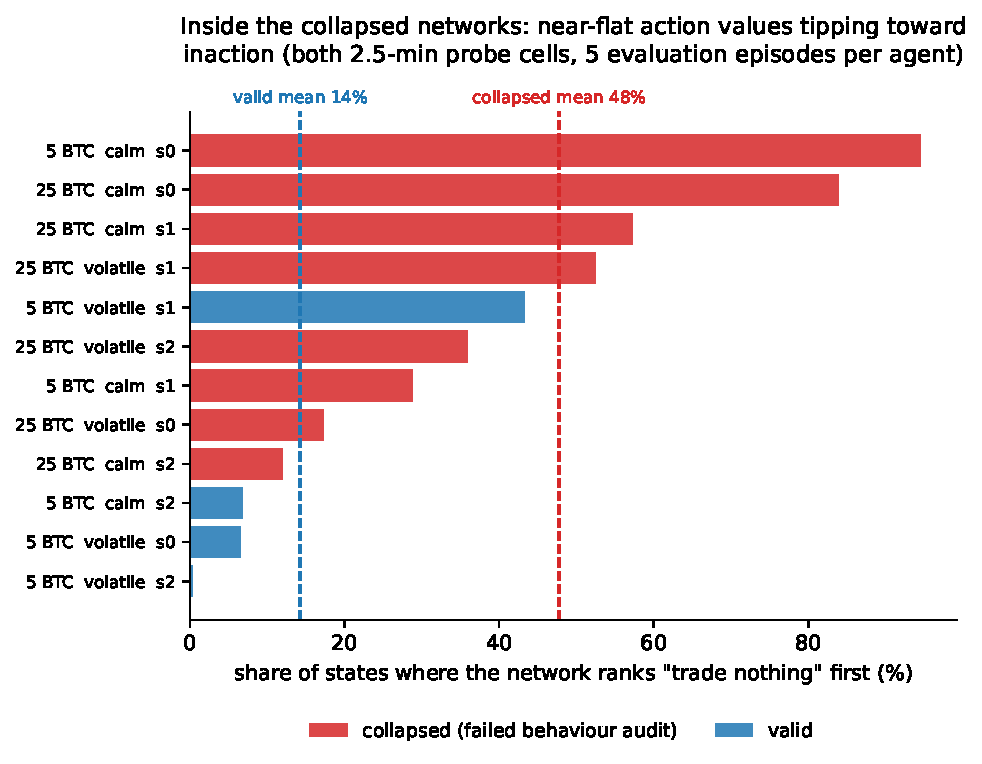
\includegraphics[width=0.8\textwidth]{fig21_q_tilt.pdf}
\caption{Inside the trained DQN networks. For each probe agent, the share of sampled
states in which the learned action values rank ``trade nothing'' first; collapsed agents
average 48\%, valid agents 14\%. The learned value separations (0.006 to 0.012) sit an
order of magnitude below the per-step reward noise, so this near-flat value surface tips
easily into systematic inaction.}
\label{fig:qtilt}
\end{figure}

\clearpage
\section{The frozen-replay track: validation results}\label{sec:l2}

On replayed historical data, where every real predictive signal is
present but the market cannot react, no agent beats TWAP consistently on any of the three
design levers (bar resolution, order size, deadline). This is the study's secondary track; the
reactive-simulator track of Sections~\ref{sec:rq1} to~\ref{sec:dqn} is the main focus. These are validation-set numbers by
design; the track's one-shot sealed exam is built and gated, and it is the track's final
verdict.

All 70 agents were evaluated on 400 validation episodes against TWAP on identical
episodes. They form 14 arms, an arm being one combination of dataset, algorithm and order
size, trained at five seeds each (Table~\ref{tab:t7}, Figure~\ref{fig:l1}). One arm is
notably agent-favourable (PPO at 96.57 BTC on 1-minute bars, pooled $-0.089$\,bps, 4/5
seeds cheaper); with 14 arms screened, approximately one such arm is expected by chance,
and it receives no special treatment: every arm sits the same sealed exam. On 10-second
bars at the 30-minute deadline agents are consistently \emph{worse} than TWAP. The DQN
deadline-leaning failure appears on this track too (six flagged runs; the L2 mirror of
Section~\ref{sec:dqn}). The size lever (Figure~\ref{fig:l2sweep}) shows benchmark costs
growing steeply with order size while no exploitable agent advantage opens at any trained
size. Full per-run detail is Appendix Table~A.2.

Two verification results from this track are reported. First, a completeness census of
all 70 agents, run before the sealed exam, found that four runs of one arm had terminated
early at 200{,}000 of the 2{,}000{,}000 training steps without saving final models. They
were excluded, the arm's provisional validation figure was withdrawn, and the four seeds
were retrained at full budget; the corrected estimate ($-0.030$\,bps) is three times weaker
than the provisional one, which is precisely why the census gate exists. Second, the track's training pipeline was verified to be bit-exactly reproducible: an
agent retrained from scratch reproduced its saved counterpart exactly, with an identical
configuration, an identical validation number to 17 decimal places, and zero difference
across the entire training curve. The sealed-exam evaluator of Section~\ref{sec:next} is
held to the same standard.

\begin{table}[h]\centering\small
\caption{Frozen-replay track validation summary, all 14 arms. Source: the 70 agents'
\texttt{meta.json} files.}
\label{tab:t7}
\resizebox{0.85\textwidth}{!}{% Auto-generated from the 70 L2 agents' meta.json files (VALIDATION data).
\begin{tabular}{llrrrr}
\toprule
panel & arm & pooled vs TWAP & cheaper & flagged & across-seed \\
 & & (bps) & seeds & seeds & $p$ \\
\midrule
1-min bars, 30-min & PPO 96.57 & -0.0890 & 4/5 & 0/5 & 0.037 \\
1-min bars, 30-min & PPO 193.13 & -0.0297 & 3/5 & 0/5 & 0.167 \\
1-min bars, 30-min & DQN 96.57 & +0.5920 & 3/5 & 1/5 & 0.796 \\
1-min bars, 30-min & DQN 193.13 & +0.0505 & 3/5 & 2/5 & 0.750 \\
\midrule
10-s bars, 30-min & PPO 96.57 & +0.1779 & 0/5 & 0/5 & 1.000 \\
10-s bars, 30-min & PPO 193.13 & +0.0740 & 1/5 & 0/5 & 0.781 \\
10-s bars, 30-min & PPO 386.27 & +0.2010 & 0/5 & 0/5 & 1.000 \\
10-s bars, 30-min & DQN 96.57 & +0.7663 & 0/5 & 1/5 & 0.884 \\
10-s bars, 30-min & DQN 193.13 & +0.1417 & 1/5 & 0/5 & 0.940 \\
10-s bars, 30-min & DQN 386.27 & +0.2049 & 1/5 & 1/5 & 0.981 \\
\midrule
10-s bars, 10-min & PPO 96.57 & +0.0066 & 3/5 & 0/5 & 0.562 \\
10-s bars, 10-min & PPO 193.13 & +0.0324 & 1/5 & 0/5 & 0.797 \\
10-s bars, 10-min & DQN 96.57 & +0.0244 & 3/5 & 1/5 & 0.672 \\
10-s bars, 10-min & DQN 193.13 & +0.1133 & 2/5 & 1/5 & 0.867 \\
\bottomrule
\end{tabular}}
\end{table}

\begin{figure}[h]\centering
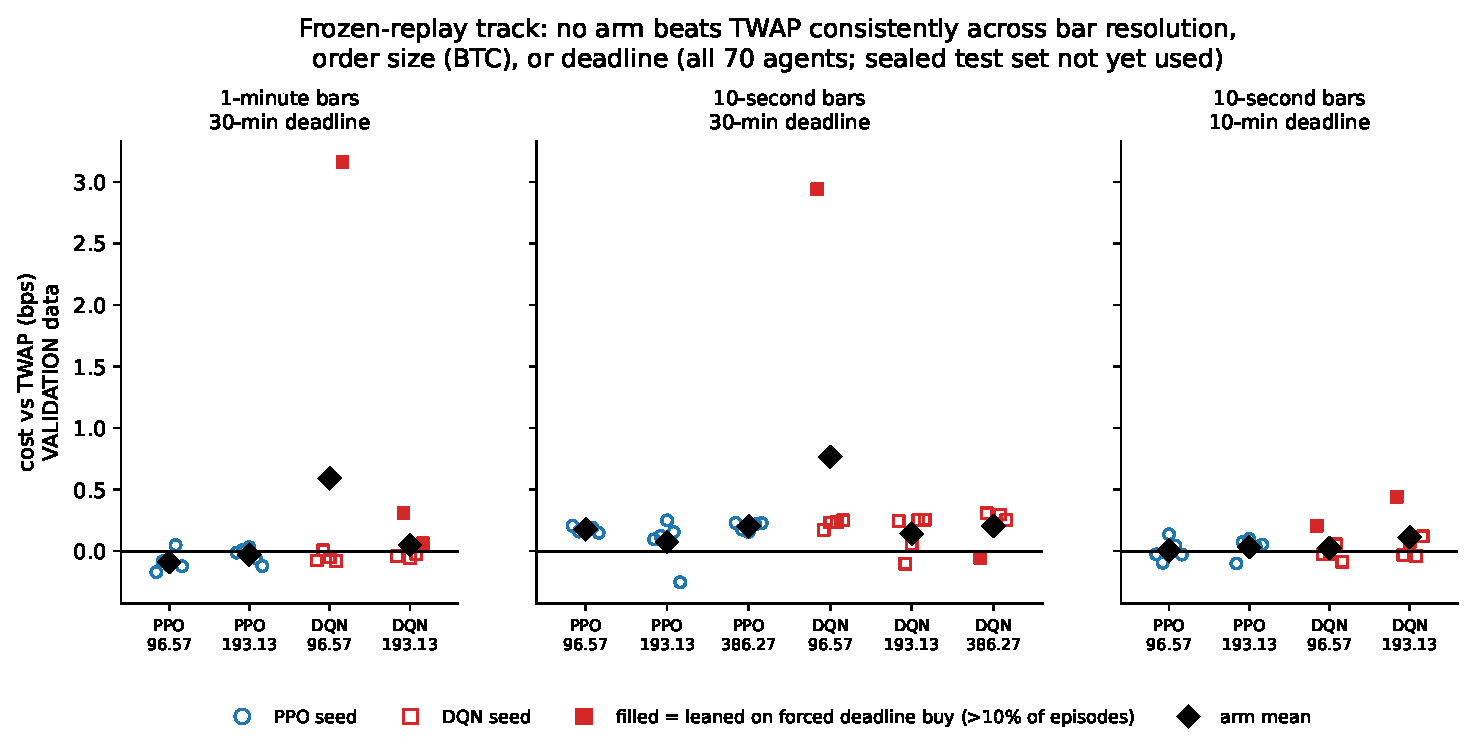
\includegraphics[width=0.98\textwidth]{l1_three_lever_null.pdf}
\caption{Frozen-replay track, the three-lever null. Each panel varies one design lever
(bar resolution, order size, deadline); points are per-seed validation results against TWAP
(negative = agent cheaper), and filled markers flag runs that leaned on the forced deadline
purchase, the frozen-replay mirror of the DQN failure. No arm beats TWAP consistently on
any lever. Validation data; the one-shot sealed exam is the track's final verdict.}
\label{fig:l1}
\end{figure}

\begin{figure}[h]\centering
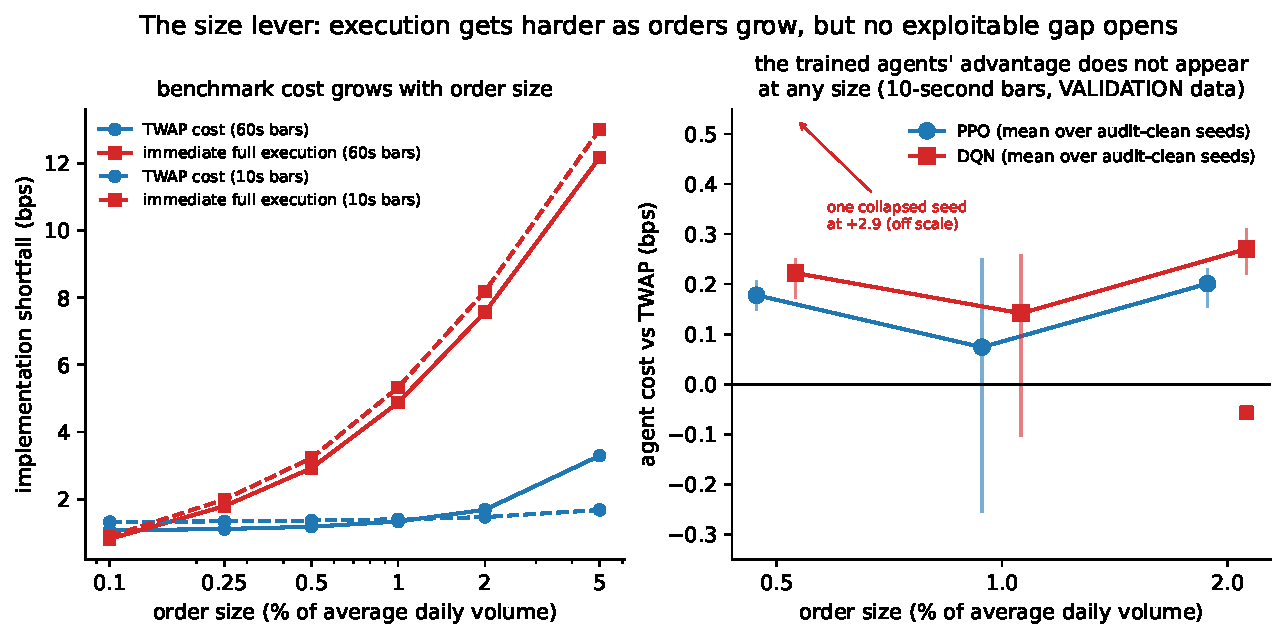
\includegraphics[width=0.98\textwidth]{l2_size_sweep.pdf}
\caption{Frozen-replay track size lever (validation data). Left, the cost of two
reference schedules versus order size as a share of average daily volume: a TWAP schedule,
and immediate full execution, meaning the entire order submitted as one market order at the
start. Immediate execution grows steeply with size while TWAP stays comparatively flat, so
execution gets harder exactly where scheduling matters. Right, the trained agents' cost
versus TWAP at each trained size on 10-second bars; no exploitable gap opens anywhere, with
collapsed seeds excluded from the means and annotated separately.}
\label{fig:l2sweep}
\end{figure}

\statusbox{A planted-signal credibility check was performed during this track's audit
phase: episodes containing a deliberately injected directional edge confirmed that the
evaluation correctly rewards policies that exploit it. The output files of that check were
not preserved, so the check will be regenerated before its result is cited quantitatively.}

\clearpage
\section{Research question 2: regime dependence}\label{sec:rq2}

Volatility regime shaped every phenomenon in this study, but not
in the direction of a usable advantage.

The development-block signal was volatile-only at the primary setting
(Figure~\ref{fig:regime}); the grid's spurious triggers were calm-only; and DQN's collapse
concentrates in calm markets. The consistent reading is that regime changes the
\emph{noise and learning landscape} (calm books recover more slowly relative to
volatility, so impact feedback differs) rather than revealing an exploitable edge in either
regime: both regimes end at the same confirmed null. The planned attribution study
(Section~\ref{sec:next}) will make the regime mechanism claim precise, and its labelling
deliberately waits for the measured-signal extension's verdict.

\section{What happens next: the pre-registered programme}\label{sec:next}

The remaining work is committed and ordered, and several of the steps below are already
registered in advance as pre-specified experiments. One step from the previous draft, the
per-episode cost-distribution analysis for the reactive track, has completed in the
meantime and now appears in Section~\ref{sec:rq1}. In order:

\begin{enumerate}
\item \textbf{Frozen-replay track sealed exam (the secondary track).} The test-set evaluator is built next; it must first
reproduce known validation numbers exactly (the same bit-exactness standard used
elsewhere), and only then is the one-shot exam of all 70 agents run: all 14 arms reported,
multiplicity stated, no re-runs. \statusbox{The evaluator is under construction and the exam has not yet been run. Its
results will convert Table~\ref{tab:t7} and Figures~\ref{fig:l1}--\ref{fig:l2sweep} into
final test-set results.}
\item \textbf{Measured-signal extension.} The one remaining experiment that can change the
headline: measure the order-flow-imbalance to future-return relationship from the L4 data
(magnitude, horizon, decay, per regime), inject exactly the measured relationship into the
reactive simulator (drift-neutral, conditioned on the background process, deconvolved from
the endogenous channel), and re-run a reduced pre-registered campaign with a fresh sealed
block. This unifies the two tracks' mechanisms in one environment.
\item \textbf{Liquidity and volume profiles} from the L4 trades (intra-day, intra-week);
also supplies the volume curve for a VWAP benchmark.
\item \textbf{Almgren-Chriss and VWAP benchmarks}, calibrated to this environment, added to
the comparison set.
\item \textbf{Attribution (research question 3).} Which order-book features drive the
agents' behaviour per regime; scheduled after the extension verdict because its labelling
depends on that outcome.
\item \textbf{Decision-frequency check.} Environment change (decision interval as a
parameter, discount factor re-derived, baselines and audit re-verified, tests), then 12
runs at 0.5-second and 2-second cadences at the primary setting.
\end{enumerate}

\clearpage
\appendix
\section{Appendix: full run-level tables}

\begin{table}[h]\centering\small
\caption{Reactive track agent configurations (base and every variant's single change).}
\label{tab:t8}
\resizebox{0.9\textwidth}{!}{% Auto-generated. Base config + each pre-registered variant's single change.
\begin{tabular}{lll}
\toprule
code & agent / variant & change from base \\
\midrule
base (PPO) & PPO, discrete actions & net 30$\times$5, lr 3e-4, reward $\times$1, n\_steps 2048, ent 0.01, 2M steps \\
base (DQN) & DQN, discrete actions & net 30$\times$5, lr 1e-4, buffer 1M, $\varepsilon$ 1.0$\to$0.01 over 25\% \\
\midrule
v1a & bigger network & net\_arch [64, 64] \\
v1b & bigger network & net\_arch [128, 128] \\
v2 & stronger feedback & reward scale $\times$100 \\
v3a & faster learning & learning rate 1e-3 \\
v3b & slower learning & learning rate 1e-4 \\
v4a & no exploration bonus & ent\_coef 0.0 \\
v4b & more exploration & ent\_coef 0.05 \\
v5 & longer rollout & n\_steps 8192 \\
v6 & v2 trained longer & reward $\times$100, 10M steps \\
v6b & v3b trained longer & lr 1e-4, 10M steps \\
w3a & combination & net [128,128] + reward $\times$100 \\
w3b & combination & lr 1e-4 + reward $\times$100 \\
d1 & DQN collapse fix & exploration\_final\_eps 0.05, anneal 0.5 \\
d2 & DQN collapse fix & reward $\times$100 + net [64,64] \\
\bottomrule
\end{tabular}}
\end{table}

\noindent\textbf{Table A.1: tuning campaign of the reactive track, all 98 runs per
seed} (source: \texttt{step5\_selection\_v3/}); the table flows over the
following pages.
\begin{center}\scriptsize% Auto-generated from step5_selection_v3 (all 98 tuning-campaign runs, per seed).
% LONGTABLE: flows across pages; include directly (no float, no resizebox).
\begin{longtable}{lllrrrrc}
\toprule
algo & regime & variant & seed & vs fixed & $p$ & vs adaptive & valid \\
\midrule
\endhead
dqn & calm & \_d1 & 0 & +0.0894 & 0.002 & +0.0895 & \textbf{NO} \\
dqn & calm & \_d1 & 1 & -0.0069 & 0.780 & -0.0068 & yes \\
dqn & calm & \_d1 & 2 & -0.0068 & 0.838 & -0.0067 & \textbf{NO} \\
dqn & calm & \_d2 & 0 & +0.1442 & 0.002 & +0.1443 & \textbf{NO} \\
dqn & calm & \_d2 & 1 & +0.1393 & 0.001 & +0.1393 & \textbf{NO} \\
dqn & calm & \_d2 & 2 & +0.0099 & 0.604 & +0.0100 & \textbf{NO} \\
dqn & volatile & \_d1 & 0 & +0.1398 & 0.157 & +0.1392 & \textbf{NO} \\
dqn & volatile & \_d1 & 1 & +0.0324 & 0.307 & +0.0318 & \textbf{NO} \\
dqn & volatile & \_d1 & 2 & -0.0396 & 0.334 & -0.0403 & yes \\
dqn & volatile & \_d2 & 0 & +0.0063 & 0.675 & +0.0057 & yes \\
dqn & volatile & \_d2 & 1 & -0.0729 & 0.032 & -0.0736 & yes \\
dqn & volatile & \_d2 & 2 & -0.0092 & 0.709 & -0.0099 & yes \\
ppo & calm & \_v1a & 0 & -0.0226 & 0.248 & -0.0225 & yes \\
ppo & calm & \_v1a & 1 & -0.0068 & 0.770 & -0.0067 & yes \\
ppo & calm & \_v1a & 2 & -0.0185 & 0.243 & -0.0184 & yes \\
ppo & calm & \_v1b & 0 & +0.0053 & 0.960 & +0.0054 & yes \\
ppo & calm & \_v1b & 1 & -0.0246 & 0.196 & -0.0245 & yes \\
ppo & calm & \_v1b & 2 & -0.0441 & 0.016 & -0.0441 & yes \\
ppo & calm & \_v2 & 0 & -0.0111 & 0.732 & -0.0110 & yes \\
ppo & calm & \_v2 & 1 & +0.0001 & 0.787 & +0.0002 & yes \\
ppo & calm & \_v2 & 2 & +0.0036 & 0.958 & +0.0036 & yes \\
ppo & calm & \_v3a & 0 & +0.0337 & 0.070 & +0.0338 & yes \\
ppo & calm & \_v3a & 1 & -0.0230 & 0.230 & -0.0229 & yes \\
ppo & calm & \_v3a & 2 & -0.0069 & 0.607 & -0.0068 & yes \\
ppo & calm & \_v3b & 0 & -0.0327 & 0.089 & -0.0326 & yes \\
ppo & calm & \_v3b & 1 & -0.0153 & 0.623 & -0.0153 & yes \\
ppo & calm & \_v3b & 2 & -0.0148 & 0.426 & -0.0147 & \textbf{NO} \\
ppo & calm & \_v4a & 0 & -0.0189 & 0.416 & -0.0188 & yes \\
ppo & calm & \_v4a & 1 & -0.0126 & 0.515 & -0.0125 & yes \\
ppo & calm & \_v4a & 2 & -0.0298 & 0.370 & -0.0298 & yes \\
ppo & calm & \_v4a & 3 & -0.0382 & 0.028 & -0.0381 & yes \\
ppo & calm & \_v4a & 4 & -0.0076 & 0.872 & -0.0075 & yes \\
ppo & calm & \_v4b & 0 & +0.0027 & 0.986 & +0.0028 & yes \\
ppo & calm & \_v4b & 1 & -0.0161 & 0.444 & -0.0161 & yes \\
ppo & calm & \_v4b & 2 & -0.0043 & 0.808 & -0.0042 & yes \\
ppo & calm & \_v5 & 0 & -0.0068 & 0.808 & -0.0067 & yes \\
ppo & calm & \_v5 & 1 & -0.0035 & 0.915 & -0.0034 & yes \\
ppo & calm & \_v5 & 2 & -0.0377 & 0.047 & -0.0376 & yes \\
ppo & calm & \_v6 & 0 & +0.0135 & 0.671 & +0.0136 & yes \\
ppo & calm & \_v6 & 1 & +0.0100 & 0.996 & +0.0100 & yes \\
ppo & calm & \_v6 & 2 & -0.0099 & 0.872 & -0.0098 & yes \\
ppo & calm & \_v6b & 0 & -0.0319 & 0.066 & -0.0318 & yes \\
ppo & calm & \_v6b & 1 & +0.0047 & 0.687 & +0.0047 & yes \\
ppo & calm & \_v6b & 2 & -0.0053 & 0.573 & -0.0052 & yes \\
ppo & calm & \_w3a & 0 & +0.0017 & 0.901 & +0.0018 & yes \\
ppo & calm & \_w3a & 1 & -0.0178 & 0.287 & -0.0177 & yes \\
ppo & calm & \_w3a & 2 & -0.0029 & 0.841 & -0.0029 & yes \\
ppo & calm & \_w3b & 0 & -0.0218 & 0.235 & -0.0217 & yes \\
ppo & calm & \_w3b & 1 & -0.0102 & 0.785 & -0.0101 & yes \\
ppo & calm & \_w3b & 2 & -0.0032 & 0.648 & -0.0031 & yes \\
ppo & volatile & \_v1a & 0 & -0.0089 & 0.803 & -0.0096 & yes \\
ppo & volatile & \_v1a & 1 & -0.0290 & 0.374 & -0.0296 & yes \\
ppo & volatile & \_v1a & 2 & +0.0232 & 0.546 & +0.0226 & \textbf{NO} \\
ppo & volatile & \_v1b & 0 & -0.0150 & 0.573 & -0.0156 & yes \\
ppo & volatile & \_v1b & 1 & -0.0436 & 0.196 & -0.0443 & yes \\
ppo & volatile & \_v1b & 2 & -0.0640 & 0.071 & -0.0646 & yes \\
ppo & volatile & \_v1b & 3 & -0.0870 & 0.020 & -0.0876 & yes \\
ppo & volatile & \_v1b & 4 & -0.0684 & 0.051 & -0.0691 & yes \\
ppo & volatile & \_v2 & 0 & -0.0501 & 0.168 & -0.0507 & yes \\
ppo & volatile & \_v2 & 1 & -0.0615 & 0.119 & -0.0621 & yes \\
ppo & volatile & \_v2 & 2 & -0.0519 & 0.186 & -0.0525 & yes \\
ppo & volatile & \_v2 & 3 & -0.0495 & 0.156 & -0.0502 & yes \\
ppo & volatile & \_v2 & 4 & -0.0150 & 0.965 & -0.0156 & yes \\
ppo & volatile & \_v3a & 0 & -0.0494 & 0.243 & -0.0500 & yes \\
ppo & volatile & \_v3a & 1 & -0.1044 & 0.012 & -0.1050 & yes \\
ppo & volatile & \_v3a & 2 & -0.0345 & 0.369 & -0.0352 & yes \\
ppo & volatile & \_v3a & 3 & -0.0798 & 0.023 & -0.0805 & yes \\
ppo & volatile & \_v3a & 4 & -0.0427 & 0.236 & -0.0433 & yes \\
ppo & volatile & \_v3b & 0 & -0.0717 & 0.047 & -0.0724 & yes \\
ppo & volatile & \_v3b & 1 & -0.1019 & 0.006 & -0.1026 & yes \\
ppo & volatile & \_v3b & 2 & -0.0759 & 0.038 & -0.0765 & yes \\
ppo & volatile & \_v3b & 3 & -0.0089 & 0.866 & -0.0095 & yes \\
ppo & volatile & \_v3b & 4 & -0.0394 & 0.344 & -0.0401 & yes \\
ppo & volatile & \_v4a & 0 & -0.0501 & 0.188 & -0.0508 & yes \\
ppo & volatile & \_v4a & 1 & -0.0764 & 0.018 & -0.0771 & yes \\
ppo & volatile & \_v4a & 2 & -0.0131 & 0.944 & -0.0137 & yes \\
ppo & volatile & \_v4b & 0 & -0.0402 & 0.266 & -0.0408 & yes \\
ppo & volatile & \_v4b & 1 & -0.0380 & 0.334 & -0.0387 & yes \\
ppo & volatile & \_v4b & 2 & -0.0231 & 0.422 & -0.0238 & yes \\
ppo & volatile & \_v4b & 3 & -0.0492 & 0.154 & -0.0498 & yes \\
ppo & volatile & \_v4b & 4 & +0.0201 & 0.682 & +0.0195 & yes \\
ppo & volatile & \_v5 & 0 & -0.0506 & 0.156 & -0.0512 & yes \\
ppo & volatile & \_v5 & 1 & -0.0211 & 0.698 & -0.0217 & yes \\
ppo & volatile & \_v5 & 2 & -0.0261 & 0.454 & -0.0267 & yes \\
ppo & volatile & \_v5 & 3 & -0.0779 & 0.056 & -0.0785 & yes \\
ppo & volatile & \_v5 & 4 & -0.0637 & 0.124 & -0.0643 & yes \\
ppo & volatile & \_v6 & 0 & -0.0245 & 0.829 & -0.0252 & yes \\
ppo & volatile & \_v6 & 1 & -0.0772 & 0.083 & -0.0778 & yes \\
ppo & volatile & \_v6 & 2 & -0.0295 & 0.608 & -0.0302 & \textbf{NO} \\
ppo & volatile & \_v6b & 0 & -0.0620 & 0.093 & -0.0627 & yes \\
ppo & volatile & \_v6b & 1 & -0.0073 & 0.976 & -0.0079 & yes \\
ppo & volatile & \_v6b & 2 & -0.0474 & 0.151 & -0.0480 & yes \\
ppo & volatile & \_w3a & 0 & -0.0602 & 0.100 & -0.0609 & yes \\
ppo & volatile & \_w3a & 1 & -0.0814 & 0.029 & -0.0821 & yes \\
ppo & volatile & \_w3a & 2 & -0.0423 & 0.470 & -0.0430 & yes \\
ppo & volatile & \_w3b & 0 & -0.0456 & 0.153 & -0.0462 & yes \\
ppo & volatile & \_w3b & 1 & +0.0471 & 0.467 & +0.0465 & \textbf{NO} \\
ppo & volatile & \_w3b & 2 & -0.0257 & 0.647 & -0.0263 & yes \\
\bottomrule
\end{longtable}\end{center}
\noindent\textbf{Table A.2: frozen-replay track, all 70 agents per seed}
(validation data; DL marks the forced deadline purchase completing more than $10\%$ of
episodes); the table flows over the following pages.
\begin{center}\scriptsize% Auto-generated: all 70 L2 agents, per seed (VALIDATION data; test columns follow
% the sealed exam). resid = share of episodes finished by the forced deadline buy.
% LONGTABLE: flows across pages; include directly (no float, no resizebox).
\begin{longtable}{llrrr}
\toprule
panel & arm & seed & vs TWAP (bps) & resid \\
\midrule
\endhead
1-min bars, 30-min & PPO 96.57 & 0 & -0.1707 & 0.8\% \\
1-min bars, 30-min & PPO 96.57 & 1 & -0.0834 & 0.2\% \\
1-min bars, 30-min & PPO 96.57 & 2 & -0.1169 & 0.5\% \\
1-min bars, 30-min & PPO 96.57 & 3 & +0.0487 & 1.0\% \\
1-min bars, 30-min & PPO 96.57 & 4 & -0.1230 & 0.5\% \\
1-min bars, 30-min & PPO 193.13 & 0 & -0.0118 & 2.0\% \\
1-min bars, 30-min & PPO 193.13 & 1 & +0.0094 & 0.2\% \\
1-min bars, 30-min & PPO 193.13 & 2 & +0.0314 & 1.8\% \\
1-min bars, 30-min & PPO 193.13 & 3 & -0.0562 & 1.2\% \\
1-min bars, 30-min & PPO 193.13 & 4 & -0.1214 & 0.8\% \\
1-min bars, 30-min & DQN 96.57 & 0 & -0.0764 & 0.0\% \\
1-min bars, 30-min & DQN 96.57 & 1 & +0.0060 & 0.5\% \\
1-min bars, 30-min & DQN 96.57 & 2 & -0.0512 & 0.8\% \\
1-min bars, 30-min & DQN 96.57 & 3 & -0.0793 & 0.0\% \\
1-min bars, 30-min & DQN 96.57 & 4 & +3.1610 & 97.8\% \textbf{DL} \\
1-min bars, 30-min & DQN 193.13 & 0 & -0.0433 & 1.5\% \\
1-min bars, 30-min & DQN 193.13 & 1 & +0.3100 & 36.8\% \textbf{DL} \\
1-min bars, 30-min & DQN 193.13 & 2 & -0.0553 & 0.2\% \\
1-min bars, 30-min & DQN 193.13 & 3 & -0.0224 & 1.5\% \\
1-min bars, 30-min & DQN 193.13 & 4 & +0.0632 & 11.8\% \textbf{DL} \\
\midrule
10-s bars, 30-min & PPO 96.57 & 0 & +0.2056 & 0.0\% \\
10-s bars, 30-min & PPO 96.57 & 1 & +0.1587 & 0.0\% \\
10-s bars, 30-min & PPO 96.57 & 2 & +0.1846 & 0.2\% \\
10-s bars, 30-min & PPO 96.57 & 3 & +0.1919 & 0.0\% \\
10-s bars, 30-min & PPO 96.57 & 4 & +0.1488 & 0.2\% \\
10-s bars, 30-min & PPO 193.13 & 0 & +0.0956 & 0.2\% \\
10-s bars, 30-min & PPO 193.13 & 1 & +0.1229 & 0.2\% \\
10-s bars, 30-min & PPO 193.13 & 2 & +0.2496 & 0.0\% \\
10-s bars, 30-min & PPO 193.13 & 3 & +0.1552 & 0.5\% \\
10-s bars, 30-min & PPO 193.13 & 4 & -0.2533 & 5.5\% \\
10-s bars, 30-min & PPO 386.27 & 0 & +0.2294 & 0.2\% \\
10-s bars, 30-min & PPO 386.27 & 1 & +0.1743 & 0.0\% \\
10-s bars, 30-min & PPO 386.27 & 2 & +0.1565 & 0.0\% \\
10-s bars, 30-min & PPO 386.27 & 3 & +0.2174 & 0.0\% \\
10-s bars, 30-min & PPO 386.27 & 4 & +0.2272 & 0.0\% \\
10-s bars, 30-min & DQN 96.57 & 0 & +2.9426 & 97.8\% \textbf{DL} \\
10-s bars, 30-min & DQN 96.57 & 1 & +0.1728 & 7.8\% \\
10-s bars, 30-min & DQN 96.57 & 2 & +0.2327 & 0.0\% \\
10-s bars, 30-min & DQN 96.57 & 3 & +0.2341 & 0.5\% \\
10-s bars, 30-min & DQN 96.57 & 4 & +0.2493 & 0.0\% \\
10-s bars, 30-min & DQN 193.13 & 0 & +0.2441 & 0.0\% \\
10-s bars, 30-min & DQN 193.13 & 1 & -0.1025 & 10.0\% \\
10-s bars, 30-min & DQN 193.13 & 2 & +0.0570 & 0.5\% \\
10-s bars, 30-min & DQN 193.13 & 3 & +0.2537 & 0.2\% \\
10-s bars, 30-min & DQN 193.13 & 4 & +0.2561 & 0.5\% \\
10-s bars, 30-min & DQN 386.27 & 0 & -0.0569 & 27.0\% \textbf{DL} \\
10-s bars, 30-min & DQN 386.27 & 1 & +0.3082 & 1.0\% \\
10-s bars, 30-min & DQN 386.27 & 2 & +0.2214 & 1.0\% \\
10-s bars, 30-min & DQN 386.27 & 3 & +0.2978 & 0.0\% \\
10-s bars, 30-min & DQN 386.27 & 4 & +0.2537 & 0.0\% \\
\midrule
10-s bars, 10-min & PPO 96.57 & 0 & -0.0262 & 0.2\% \\
10-s bars, 10-min & PPO 96.57 & 1 & -0.0946 & 0.2\% \\
10-s bars, 10-min & PPO 96.57 & 2 & +0.1367 & 0.0\% \\
10-s bars, 10-min & PPO 96.57 & 3 & +0.0450 & 0.0\% \\
10-s bars, 10-min & PPO 96.57 & 4 & -0.0280 & 0.5\% \\
10-s bars, 10-min & PPO 193.13 & 0 & -0.1008 & 1.0\% \\
10-s bars, 10-min & PPO 193.13 & 1 & +0.0741 & 1.0\% \\
10-s bars, 10-min & PPO 193.13 & 2 & +0.0985 & 1.5\% \\
10-s bars, 10-min & PPO 193.13 & 3 & +0.0373 & 1.5\% \\
10-s bars, 10-min & PPO 193.13 & 4 & +0.0529 & 0.5\% \\
10-s bars, 10-min & DQN 96.57 & 0 & +0.2065 & 26.2\% \textbf{DL} \\
10-s bars, 10-min & DQN 96.57 & 1 & -0.0264 & 0.0\% \\
10-s bars, 10-min & DQN 96.57 & 2 & -0.0275 & 0.0\% \\
10-s bars, 10-min & DQN 96.57 & 3 & +0.0553 & 0.2\% \\
10-s bars, 10-min & DQN 96.57 & 4 & -0.0861 & 1.8\% \\
10-s bars, 10-min & DQN 193.13 & 0 & +0.4411 & 48.8\% \textbf{DL} \\
10-s bars, 10-min & DQN 193.13 & 1 & -0.0312 & 3.0\% \\
10-s bars, 10-min & DQN 193.13 & 2 & +0.0772 & 0.0\% \\
10-s bars, 10-min & DQN 193.13 & 3 & -0.0401 & 0.0\% \\
10-s bars, 10-min & DQN 193.13 & 4 & +0.1193 & 0.0\% \\
\bottomrule
\end{longtable}\end{center}
\clearpage

\clearpage
\section{Appendix: provenance}\label{sec:provenance}

Every number in this chapter is generated by script from primary result files that are
version-controlled with the project repository under \texttt{results\_archive/} (reactive
track in \texttt{qrm/}, frozen replay in \texttt{l2/}; the paths below are relative to
\texttt{results\_archive/}). The archive holds every scored evaluation, behaviour audit,
run configuration, training curve, trained model, and per-episode cost record, so every
figure and table in this document can be regenerated from it. Raw exchange data and the
derived training datasets are excluded for size; the repository's pipeline scripts rebuild
them from Hyperliquid's public data archive.

\begin{center}\small
\begin{tabular}{ll}
\toprule
result & source of truth \\
\midrule
Primary campaign (T\ref{tab:t1}, F\ref{fig:regime}, F\ref{fig:dqncollapse}) & \texttt{qrm/step5\_v3/} \\
Tuning + selection (T\ref{tab:t2}, A.1, F\ref{fig:forestv}, F\ref{fig:forestc}) & \texttt{qrm/step5\_selection\_v3/} \\
Sealed confirmations (T\ref{tab:t3}, F\ref{fig:headline}) & \texttt{qrm/step5\_confirm\_\{v3a,v1b\}/} \\
Sweeps + grid (F\ref{fig:size}, F\ref{fig:grid}, T\ref{tab:t4}) & \texttt{qrm/step5\_sweep\_*, qrm/step5\_grid\_*/} \\
Replication ladder (F\ref{fig:ladder}, T\ref{tab:t12}) & \texttt{qrm/step5\_esc\_*, qrm/step5\_xblock\_*/} \\
DQN probe + d3 (F\ref{fig:dqnsettings}, T\ref{tab:t11}) & \texttt{qrm/step5\_dqnprobe\_*, qrm/step5\_d3\_*/} \\
Q-value diagnostic (F\ref{fig:qtilt}) & \texttt{reports/diagnostics/dqn\_q\_flatness.json} (repository path) \\
Environment gates (T\ref{tab:t5}) & \texttt{qrm/step4\_gates\_v3.json, qrm/step3g/} \\
Frozen-replay agents (T\ref{tab:t7}, A.2, F\ref{fig:l1}) & \texttt{l2/runs/, l2/runs\_10s/, l2/runs\_10s\_10min/} \\
Frozen-replay benchmark sweep (F\ref{fig:l2sweep}) & \texttt{l2/size\_sweep\_results.json} \\
Learning curves (F\ref{fig:curves}) & \texttt{qrm/runs\_*/} per-run \texttt{curve.json} \\
Drift confound, before/after (F\ref{fig:drift}) & \texttt{qrm/SUPERSEDED\_step5\_v2/} (pre-fix), \texttt{qrm/step5\_v3/} \\
Per-episode distributions (F\ref{fig:dist}, F\ref{fig:paired}, T\ref{tab:t6}) & \texttt{qrm/per\_episode\_v3/} \\
\bottomrule
\end{tabular}
\end{center}

\end{document}
